\chapter{Landasan Teori}
\label{chap:teori}

\section{SharIF Judge}
\label{sec:2:sharif}

SharIF Judge (dengan IF kapital) adalah modifikasi cabang dari Sharif Judge (dengan if kecil), sebuah \textit{online judge} gratis untuk bahasa pemrograman C, C++, Java dan Python yang diciptakan oleh Mohammad Javad Naderi dengan \textit{framework} CodeIgniter dan Bash\cite{sharif}. Modifikasi ini dilakukan oleh Stillmen Vallian untuk menyesesuaikan Sharif Judge terhadap kebutuhan-kebutuhan spesifik Teknik Informatika Unpar. SharIF Judge digunakan pada beberapa mata kuliah pemrograman Teknik Informatika Unpar untuk mempermudah proses pengumpulan dan penilaian kode program. \cite{stillmen:sharif}

\subsection{Instalasi}
\label{subs:2:instalasi}
Untuk menjalankan SharIF Judge, diperlukan sebuah \textit{server} Linux yang memenuhi prasyarat berikut ini:
\begin{itemize}
    \item \textit{Webserver} dengan PHP versi 5.3 atau lebih
    \item PHP Command Line Interface (CLI)
    \item \textit{Database} MySql atau PostgreSql
    \item PHP memiliki akses untuk menjalankan \textit{shell commands} dengan fungsi \verb|shell_exec|
    \item Kemampuan untuk mengompilasi dan menjalankan kode yang dikumpulkan (\texttt{gcc}, \texttt{g++}, \texttt{javac}, \texttt{java}, \texttt{python2} dan \texttt{python3})
    \item Perl
\end{itemize}

Pada perangkat yang sudah memenuhi prasyarat, instalasi SharIF Judge dapat dilakukan dengan cara berikut ini:
\begin{enumerate}
    \item Unduh versi terakhir dari Sharif Judge dan menempatkannya pada direktori publik.
    \item Pindahkan folder \texttt{system} dan \texttt{application} ke luar direktori publik. Kemudian simpan alamatnya pada \texttt{index.php}.
    \item Buat sebuah \textit{Database} MySql atau PostgreSql.
    \item Atur pengaturan koneksi \textit{database} pada \texttt{application/config/database.php}.
    \item Atur agar direktori \texttt{application/cache/Twig} dapat ditulis oleh php.
    \item Buka halaman utama SharIF Judge pada \textit{browser} dan ikuti proses instalasi.
    \item Log in dengan akun admin
    \item Pindahkan folder \texttt{tester} dan \texttt{assignments} ke luar direktori publik. Kemudian simpan alamatnya pada halaman pengaturan.
\end{enumerate}


\subsection{Fitur-fitur}
\label{subs:2:fitur}

Pada SharIF Judge, pengguna terbagi menjadi beberapa \textit{role}. \textit{Role} yang tersedia pada SharIF Judge adalah sebagai berikut:
\begin{enumerate}
    \item \textit{admin}
    \item \textit{head instructor}
    \item \textit{instructor}
    \item \textit{student}
\end{enumerate}

Halaman dan tampilan yang tersedia pada pengguna SharIF Judge bergantung pada \textit{role} akun yang digunakan pengguna tersebut. Pada gambar \ref{fig:2:usecased}, terdapat Use Case Diagram untuk setiap \textit{role} yang tersedia. 

\begin{figure}[H]
	\centering  
	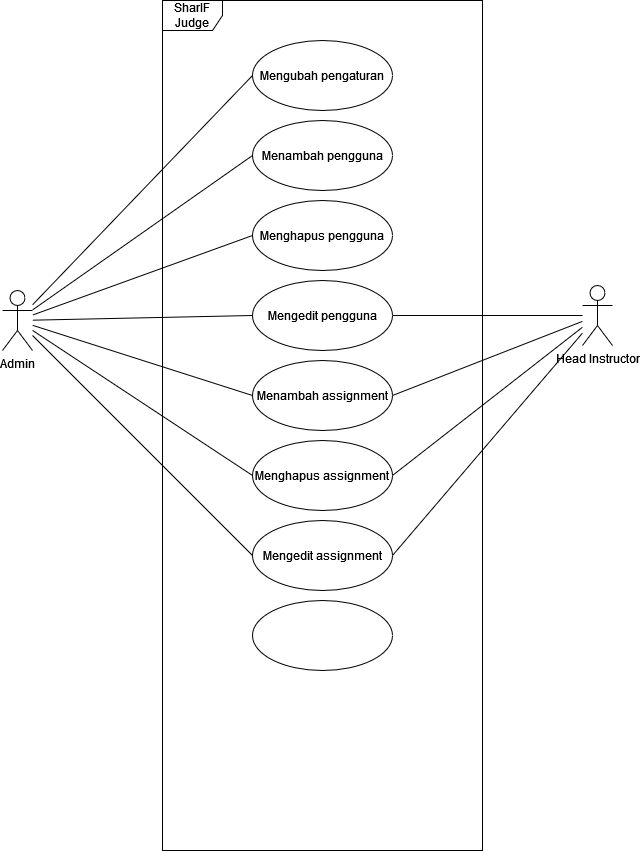
\includegraphics[scale=0.4]{Diagram/Use Case.png}  
	\caption{Use Case Diagram SharIF Judge}
	\label{fig:2:usecased} 
\end{figure} 

\section{CodeIgniter 3}
\label{sec:2:codeigniter} 

CodeIgniter adalah sebuah \textit{framework} untuk membangun situs web menggunakan PHP. Tujuan utamanya adalah untuk mempercepat pembuatan proyek dengan menyediakan \textit{library} yang lengkap untuk fungsi-fungsi yang umum digunakan, serta antarmuka yang sederhana dan struktur yang logis untuk mengakses \textit{library} tersebut \cite{codeigniter}.

\begin{figure}[H]
	\centering  
	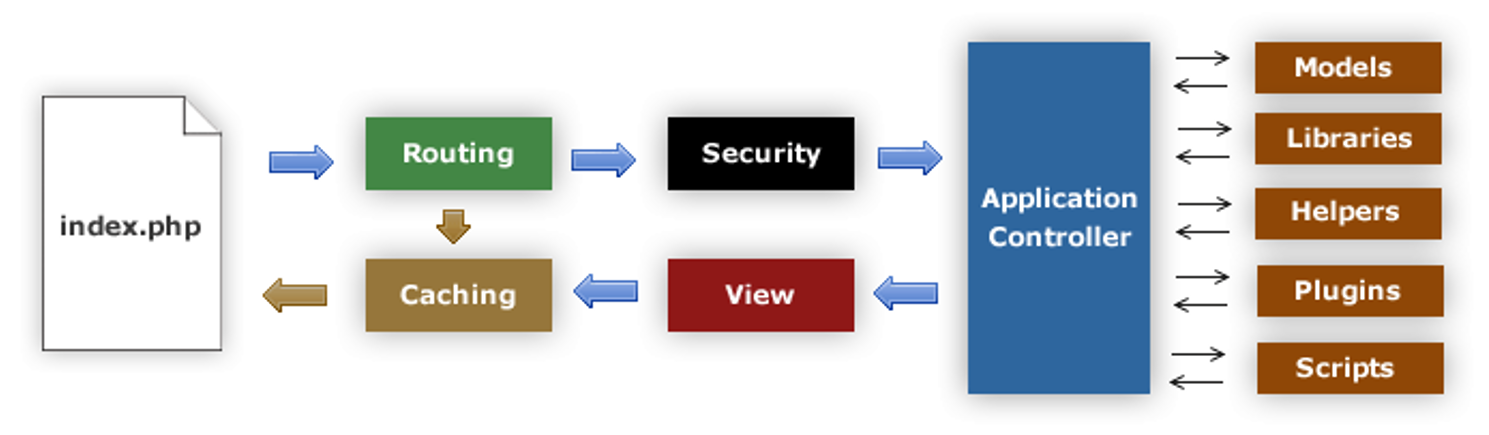
\includegraphics[scale=0.3]{ci-flowchart}  
	\caption{\textit{Flow Chart} CodeIgniter}
	\label{fig:2:ciflowchart} 
\end{figure} 

Gambar~\ref{fig:2:ciflowchart} mengilustrasikan bagaimana data mengalir pada sistem CodeIgniter.

\begin{enumerate}
	\item \textit{File} index.php berfungsi sebagai \textit{front controller}, menginisialisasi \textit{resource} utama untuk menjalankan CodeIgniter.
	\item Router meneliti \textit{request} HTTP dan menentukan apa yang harus dilakukan.
	\item Jika terdapat \textit{file} \textit{cache}, maka langsung dikirimkan ke \textit{browser}.
	\item Sebelum \textit{controller} dimuat, seluruh \textit{request} HTTP dan data dari user disaring terlebih dahulu untuk keamanan.
	\item \textit{Controller} memuat \textit{model}, \textit{library} utama, dan  \textit{resource} lainnya yang diperlukan.
	\item \textit{View} akhir lalu dikirim ke browser untuk dilihat. \textit{Cache} akan dibuat terlebih dahulu bila diaktifkan. 
\end{enumerate}

\subsection{Model-View-Controller}
\label{subs:2:cimvc} 
CodeIgniter menggunakan pola arsitektur MVC (\textit{Model-View-Controller}) sebagai dasarnya. MVC memisahkan proses logika aplikasi dari presentasi. Dengan demikian, halaman web dapat memuat sedikit \textit{script} karena presentasinya terpisah dari \textit{scripting} PHP.

\subsubsection{Model}
\textit{Model} merepresentasikan struktur data. Biasanya \textit{model} memiliki fungsi-fungsi yang membantu dalam mengambil, memasukkan, dan memperbarui informasi pada \textit{database}. Pada CodeIgniter, \textit{model} adalah sebuah kelas yang mengekstensi \verb|CI_Model| dan terletak di direktori \verb|application/models/|.

\begin{lstlisting}[language=php, caption=Contoh \textit{model}, label=kode:2:cimodel]
class Blog_model extends CI_Model {

        public $title;
        public $content;
        public $date;

        public function get_last_ten_entries()
        {
                $query = $this->db->get('entries', 10);
                return $query->result();
        }

        public function insert_entry()
        {
                $this->title    = $_POST['title']; // please read the below note
                $this->content  = $_POST['content'];
                $this->date     = time();

                $this->db->insert('entries', $this);
        }

        public function update_entry()
        {
                $this->title    = $_POST['title'];
                $this->content  = $_POST['content'];
                $this->date     = time();

                $this->db->update('entries', $this, array('id' => $_POST['id']));
        }

}
\end{lstlisting}

Kode \ref{kode:2:cimodel} merupakan contoh sebuah kelas \textit{model} pada CodeIgniter. Kelas tersebut mengekstensi \verb|CI_Model| dan memiliki fungsi untuk mengambil, memasukkan, dan memperbarui \textit{database}.
	
\subsubsection{View}
\textit{View} adalah informasi yang ditampilkan kepada pengguna. Pada CodeIgniter, \textit{view} merupakan sebuah halaman web atau sebagian dari halaman web yang terletak di direktori \verb|application/view/|.

\begin{lstlisting}[language=php, caption=Contoh \textit{view}, label=kode:2:ciview]
<html>
<head>
        <title>My Blog</title>
</head>
<body>
        <h1>Welcome to my Blog!</h1>
</body>
</html>
\end{lstlisting}

Kode \ref{kode:2:ciview} merupakan contoh sebuah \textit{view}. \textit{View} pada CodeIgniter harus dipanggil melalui \textit{Controller} dan tidak pernah dipanggil secara langsung.
	
\subsubsection{Controller}
\textit{Controller} adalah perantara dari \textit{model} dan \textit{view}, serta \textit{resource} lainnya yang diperlukan untuk memproses \textit{request} HTTP dan menghasilkan sebuah halaman web. Pada CodeIgniter, \textit{controller} adalah sebuah kelas yang mengekstensi \verb|CI_Controller| dan terletak di direktori \verb|application/controllers/|.

\begin{lstlisting}[language=php, caption=Contoh \textit{controller}, label=kode:2:cicontroller]
class Blog extends CI_Controller {

        public function index()
        {
                echo 'Hello World!';
        }

        public function comments()
        {
                echo 'Look at this!';
        }
}
\end{lstlisting}

Kode \ref{kode:2:cimodel} merupakan contoh sebuah kelas \textit{controller} pada CodeIgniter. Kelas tersebut mengekstensi \verb|CI_Controller| dan memiliki fungsi \verb|index()| dan \verb|comments()|. Fungsi \verb|index()| akan dipanggil secara otomatis jika tidak ada fungsi lain yang dipanggil. 

\begin{lstlisting}[language=php, caption=Contoh memuat \textit{model} dan menampilkan \textit{view}, label=kode:2:cimodelview]
class Blog_controller extends CI_Controller {

        public function blog()
        {
                $this->load->model('blog');

                $data['query'] = $this->blog->get_last_ten_entries();

                $this->load->view('blog', $data);
        }
}
}
\end{lstlisting}

Pada CodeIgniter, \textit{model} dan \textit{view} hanya dapat dimuat melalui controller. Pada contoh kode \ref{kode:2:cimodelview}, fungsi \verb|blog()| pada \textit{controller} memuat \textit{model} untuk mengambil data dari \textit{database}, lalu menampilkan \textit{view} yang memuat data tersebut. 

\subsection{URL CodeIgniter}
\label{subs:2:ciurl}

URL pada CodeIgniter menggunakan \textit{segment-based approach} yang dirancang untuk lebih mudah dibaca oleh \textit{search engine} dan manusia. Berikut ini adalah contoh sebuah URL pada CodeIgniter:
\begin{center}
    \verb|example.com/class/function/ID|    
\end{center}
\begin{itemize}
	\item Bagian pertama, \verb|class| merepresentasikan kelas \textit{controller} yang akan dipanggil.
	\item Bagian kedua,  \verb|function| merepresentasikan fungsi yang akan dipanggil.
	\item Bagian ketiga dan seterusnya, \verb|ID| merepresentasikan variabel yang akan digunakan.
\end{itemize}

\section{Twig}
\label{sec:2:twig}

Twig adalah sebuah \textit{template engine} untuk PHP. Sebuah \textit{template} Twig memuat \textit{variable} atau \textit{expression} yang nantinya akan diubah menjadi \textit{value} saat template dievaluasi, serta \textit{tag} yang mengontrol logika template \cite{twig}.

\begin{lstlisting}[language=php, caption=Contoh template Twig, label=kode:2:twig]
<!DOCTYPE html>
<html>
    <head>
        <title>My Webpage</title>
    </head>
    <body>
        <ul id="navigation">
        
            <li><a href="{{ item.href }}">{{ item.caption }}</a></li>
        
        </ul>

        <h1>My Webpage</h1>
        {{ a_variable }}
    </body>
</html>
\end{lstlisting}

Kode \ref{kode:2:twig} merupakan contoh sebuah template Twig. Terdapat dua jenis \textit{delimiter}, yaitu \verb|| dan \verb|{{ ... }}|. \textit{Delimiter} \verb|| digunakan untuk menjalankan \textit{statement} seperti \verb|for| dan \verb|if|, sementara \textit{delimiter} \verb|{{ ... }}| digunakan untuk menampilkan nilai dari \textit{variable} atau \textit{expression}.

\section{Bash}
\label{sec:2:shell}
Bourne Again SHell (Bash) program yang disempurnakan dari \textit{shell} Unix pertama yang diciptakan oleh Steve Bourne \cite{linux}. \textit{Shell} adalah sebuah program pada sistem operasi Unix yang menerima perintah tertulis dan mengirimnya ke sistem operasi untuk dijalankan. 

\textit{Shell script} adalah sebuah \textit{file} yang menyimpan rangkaian perintah. \textit{Shell} akan membaca \textit{file} tersebut dan menjalankan rangkaian perintah seperti jika perintah tersebut dimasukkan secara langsung pada \textit{command line}. Keunikan dari \textit{shell} adalah kemampuannya sebagai \textit{command line interface} dan sebagai  \textit{scripting language interpreter}. Artinya, hal yang dapat dilakukan melalui \textit{command line} dapat dilakukan sebagai \textit{script}, dan hal yang dapat dilakukan sebagai \textit{script} dapat dilakukan melalui \textit{command line}.

Berikut ini merupakan beberapa \textit{command} yang tersedia pada Bash:

\begin{itemize}
    \item \verb|grep regexp| \\ Mencari pola yang sesuai dengan \verb|regexp|, kemudian mencetak seluruh baris yang sesuai dengan pola tersebut.
    \item \verb|sed s/regexp/replacement/| \\ Mencari pola yang sesuai dengan \verb|regexp| dan menggantinya dengan \verb|replacement|.
\end{itemize}

\section{PDF.js}
\label{sec:2:pdfjs} 
PDF.js adalah sebuah library JavaScript yang berfungsi untuk menampilkan \textit{file} Portable Document Format (PDF) menggunakan HTML5 \textit{Canvas} \cite{pdfjs}. PDF.js terdiri dari 3 lapisan:

\begin{itemize}
	\item \textit{\textbf{Core}} merupakan bagian dimana proses \textit{parse} dan \textit{interpret} dilakukan terhadap \textit{binary} PDF.
	\item \textit{\textbf{Display}} mengambil \textit{layer} \textit{core} sebagai API yang lebih mudah digunakan untuk menampilkan PDF dan mengambil informasi lainnya dari sebuah dokumen.
	\item \textit{\textbf{Viewer}} membangun \textit{layer} \textit{display} sebagai halaman website dengan \textit{user interface} yang dapat ditampilkan di browser.
\end{itemize}

\begin{lstlisting}[language=php, caption=Contoh kode untuk menggunakan PDF.js, label=kode:2:pdfjs]
<!DOCTYPE html>
<html>
    <iframe src="/web/viewer.html?file=sample.pdf"></iframe>
</html>
\end{lstlisting}

Salah satu cara untuk menampilkan \textit{file} PDF menggunakan PDF.js adalah dengan \textit{embed} layer \textit{viewer} yang sudah tersedia melalui \verb|web/viewer.js| pada sebuah \verb|iframe|. Kode \ref{kode:2:pdfjs} merupakan contoh kode \textit{embed} PDF.js untuk menampilkan sebuah file PDF contoh \verb|sample.pdf|.

\section{Ace}
\label{sec:2:ace} 
Ace adalah sebuah library JavaScript yang berfungsi sebagai \textit{code editor}.
Ace memiliki fitur-fitur yang dapat ditemukan di \textit{code editor} pada umumnya \cite{ace}. Berikut ini merupakan beberapa fitur utama dari Ace: 

\begin{itemize}
    \item \textit{Syntax highlighting} untuk bahasa pemrograman.
    \item \textit{Indent} dan \textit{outdent} otomatis.
    \item Kemampuan \textit{cut}, \textit{copy}, dan \textit{paste}.
    \item Kemampuan \textit{drag and drop} teks menggunakan mouse.
\end{itemize}

Berikut ini adalah beberapa kelas yang terdapat pada Ace:

\begin{itemize}
    \item \verb|Ace| \\ Kelas utama yang digunakan mempersiapkan Ace pada browser. Salah satu fungsi yang dimiliki:
        \begin{itemize}
            \item \texttt{edit(String | DOMElement el)} \\ \textit{Embed} Ace pada elemen yang disediakan.
        \end{itemize}
    \item \verb|Anchor| \\ Menangani posisi \textit{pointer} pada dokumen.
    \item \verb|BackgroundTokenizer| \\ Bekerja di latar belakang untuk melakukan tokenisasi pada dokumen saat ini dan menyimpan baris yang sudah ditokenisasi sebagai \textit{cache}.
    \item \verb|Document| \\ Menyimpan teks dari dokumen. 
    \item \verb|EditSession| \\ Menyimpan seluruh \textit{state} untuk \verb|Editor| dan menyediakan cara untuk mengubahnya dengan mudah. Beberapa fungsi yang dimiliki:
        \begin{itemize}
            \item \verb|getMode()| \\ Mengembalikan mode \textit{syntax highlighting} editor yang sedang digunakan.
            \item \verb|setMode()| \\ Mengubah mode \textit{syntax highlighting} editor.
        \end{itemize}
    \item \verb|Editor| \\ \textit{Entry point} utama untuk seluruh kegunaan Ace. Beberapa fungsi yang dimiliki:
        \begin{itemize}
            \item \verb|getReadOnly()| \\ Mengembalikan \verb|true| jika editor sedang menggunakan pengaturan \textit{read-only}.
            \item \verb|getTheme()| \\ Mengembalikan alamat tema editor yang sedang digunakan.
            \item \verb|getValue()| \\ Mengembalikan isi teks editor.
            \item \verb|setReadOnly(Boolean readOnly)| \\ Mengubah pengaturan \textit{read-only}.
            \item \verb|setTheme(String style)| \\ Mengubah tema editor.
            \item \verb|setValue(String val, Number cursorPos)| \\ Mengubah isi teks editor.
        \end{itemize}
    \item \verb|Range| \\ Mengindikasi sebuah daerah pada editor.
    \item \verb|Scrollbar| \\ Menangani \textit{scrollbar} editor.
    \item \verb|Search| \\ Menangani seluruh operasi pencarian teks pada dokumen.
    \item \verb|Selection| \\ Menyimpan posisi kursor dan seleksi teks pada editor.
    \item \verb|TokenIterator| \\ Menyediakan fungsi untuk membaca dokumen sebagai aliran token.
    \item \verb|Tokenizer| \\ Menerima sejumlah aturan dan membuat \verb|Tokenizer|.
    \item \verb|UndoManager| \\ Menangani fungsi \textit{undo} pada editor.
    \item \verb|VirtualRenderer| \\ Menggambar tampilan yang terlihat di layar.
\end{itemize}


\begin{lstlisting}[language=php, caption=Contoh kode untuk menggunakan Ace, label=kode:2:ace]
<!DOCTYPE html>
<html>
<head>
<title>ACE in Action</title>
</head>
<body>

<div id="editor">
function foo(items) {
    var x = "All this is syntax highlighted";
    return x;
}
</div>
    
<script src="/ace-builds/src-noconflict/ace.js" type="text/javascript" charset="utf-8"></script>
<script>
    var editor = ace.edit("editor");
    editor.setTheme("ace/theme/monokai");
    editor.session.setMode("ace/mode/javascript");
</script>
</body>
</html>
\end{lstlisting} 

Kode \ref{kode:2:ace} merupakan contoh kode untuk menempatkan editor Ace pada sebuah elemen \verb|div| dengan id \verb|editor|. Terdapat berbagai konfigurasi pada Ace, pada contoh ini digunakan tema \textit{monokai} dan mode \textit{syntax highlighting} untuk JavaScript.




